\documentclass[tikz,border=15pt]{standalone}
\usetikzlibrary{decorations.pathreplacing, arrows.meta}
\begin{document}
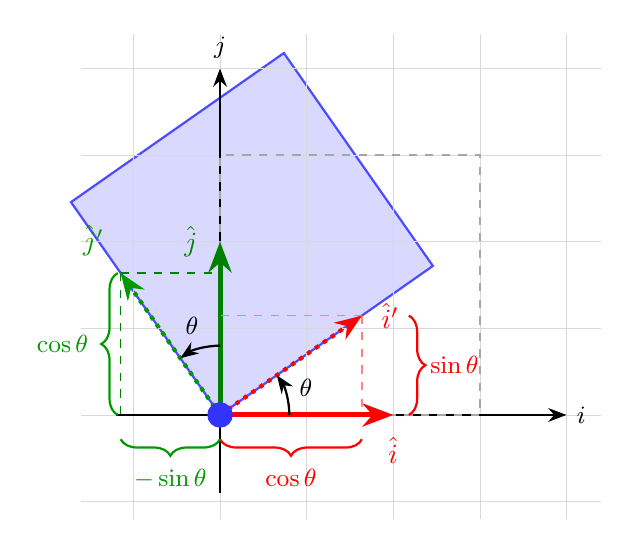
\begin{tikzpicture}[>=Stealth, scale=2.2]

    \def\ang{35}

    % ── Rotated square FIRST (behind everything) ─────────────────────────────
    \begin{scope}[rotate=\ang]
        \filldraw[fill=blue!15, draw=blue!70, thick] (0,0) rectangle (1.5,1.5);
    \end{scope}

    % ── Grid ─────────────────────────────────────────────────────────────────
    \draw[help lines, step=0.5, gray!30] (-0.8,-0.6) grid (2.2,2.2);

    % ── Axes ─────────────────────────────────────────────────────────────────
    \draw[->, thick, black] (-0.6, 0) -- (2.0, 0) node[right, font=\small] {$i$};
    \draw[->, thick, black] (0, -0.45) -- (0, 2.0) node[above, font=\small] {$j$};

    % Origin label
    % \node[below left, font=\small, green!60!black] at (0,0) {$O$};

    % ── Original square: dashed, bottom-left at origin ───────────────────────
    \draw[dashed, thick, gray!70] (0,0) rectangle (1.5,1.5);

    % ── Original unit vectors i, j ───────────────────────────────────────────
    \draw[->, very thick, red, line width=1.8pt] (0,0) -- (1,0)
        node[below=4pt, font=\normalsize] {$\hat{i}$};
    \draw[->, very thick, green!50!black, line width=1.8pt] (0,0) -- (0,1)
        node[left=4pt, font=\normalsize] {$\hat{j}$};

    % ── Coordinates ──────────────────────────────────────────────────────────
    \coordinate (Ip)  at ({cos(\ang)},  {sin(\ang)});
    \coordinate (Jp)  at ({-sin(\ang)}, {cos(\ang)});
    \coordinate (IpX) at ({cos(\ang)},  0);
    \coordinate (IpY) at (0, {sin(\ang)});
    \coordinate (JpX) at ({-sin(\ang)}, 0);
    \coordinate (JpY) at (0, {cos(\ang)});

    % ── Projection dashed lines ───────────────────────────────────────────────
    \draw[dashed, red!50,          thin] (Ip) -- (IpX);
    \draw[dashed, red!50,          thin] (Ip) -- (IpY);
    \draw[dashed, green!50!black,  thin] (Jp) -- (JpX);
    \draw[dashed, green!50!black,  thin] (Jp) -- (JpY);

    % ── New unit vectors i', j' ───────────────────────────────────────────────
    \draw[->, red, very thick, line width=1.5pt, dotted] (0,0) -- (Ip)
        node[right=3pt, font=\normalsize, red] {$\hat{i}'$};
    \draw[->, green!60!black, very thick, line width=1.5pt, dotted] (0,0) -- (Jp)
        node[above left=2pt, font=\normalsize, green!60!black] {$\hat{j}'$};

    % ── Angle arcs ───────────────────────────────────────────────────────────
    \draw[->, thick] (0.40, 0) arc (0:\ang:0.40);
    \node[font=\small] at ({0.52*cos(\ang/2)}, {0.52*sin(\ang/2)}) {$\theta$};

    \draw[->, thick] (0, 0.40) arc (90:{90+\ang}:0.40);
    \node[font=\small] at ({0.54*cos(90+\ang/2)}, {0.54*sin(90+\ang/2)}) {$\theta$};

    % ── Origin dot ───────────────────────────────────────────────────────────
    \filldraw[blue!80] (0,0) circle (2pt);

    % ════════════════════════════════════════════════════════════════════════
    % CURLY BRACES
    % ════════════════════════════════════════════════════════════════════════

    % RED — cos θ: x-axis, brace below, left→right, tooth points down
    \draw[decorate, decoration={brace, amplitude=6pt, mirror},
          thick, red]
        (0, -0.14) -- ({cos(\ang)}, -0.14)
        node[midway, below=7pt, font=\small, red] {$\cos\theta$};

    % RED — sin θ: y-axis, brace on RIGHT side, bottom→top
    \draw[decorate, decoration={brace, amplitude=6pt, mirror},
          thick, red]
        (1.09, 0) -- (1.09, {sin(\ang)})
        node[midway, right=4pt, font=\small, red] {$\sin\theta$};

    % GREEN — -sin θ: negative x-axis, brace below, left→right, tooth points down
    \draw[decorate, decoration={brace, amplitude=6pt, mirror},
          thick, green!60!black]
        ({-sin(\ang)}, -0.14) -- (0, -0.14)
        node[midway, below=7pt, font=\small, green!60!black] {$-\sin\theta$};

    % GREEN — cos θ: y-axis, brace on LEFT side, bottom→top
    \draw[decorate, decoration={brace, amplitude=6pt},
          thick, green!60!black]
        (-0.59, 0) -- (-0.59, {cos(\ang)})
        node[midway, left=7pt, font=\small, green!60!black] {$\cos\theta$};

\end{tikzpicture}
\end{document}